\documentclass[aspectratio=169,10pt]{beamer}
\usepackage{../common/beamer_theme_bio}

\title{\textbf{Biostatistiques Appliquées}}
\subtitle{Chapitre II : Analyse de Variance Hiérarchisée (Nested ANOVA) \& Plans Emboîtés}
\author{\textbf{Dr. Sarra BENMOUMOU (Ph.D.)}}
\institute{
  Faculté des Sciences --- Département de Biologie\\
  Master 2 : Biochimie Appliquée\\
  \textbf{Université M'Hamed Bougara de Boumerdès (UMBB)}
}
\date{Année Universitaire 2024 -- 2025}

\begin{document}

\begin{frame}[plain]
  \titlepage
\end{frame}

\begin{frame}{Plan Détaillé du Chapitre II}
  \tableofcontents
\end{frame}

% ========================================================
\section{Concepts des Facteurs Emboîtés}
% ========================================================

\begin{frame}{Pourquoi des Plans Hiérarchisés en Biologie ?}
  \begin{columns}[onlytextwidth, T]
    \begin{column}{0.48\linewidth}
      \begin{conceptbox}{Facteurs Croisés (Rappel)}
        Toutes les combinaisons possibles existent :
        \begin{equation*}
          \text{Dose } (1, 2, 3) \times \text{ Sexe } (\text{M}, \text{F})
        \end{equation*}
        Un animal mâle peut recevoir n'importe quelle dose.
      \end{conceptbox}
    \end{column}
    \begin{column}{0.48\linewidth}
      \begin{conceptbox}{Facteurs Hiérarchisés ($B \subset A$)}
        Les modalités de B sont \textbf{uniques} à un niveau donné de A :
        \begin{equation*}
          \text{Flacon } j \subset \text{ Lot Industriel } i
        \end{equation*}
        Le flacon n$^\circ$1 prélevé dans le Lot A n'a \textbf{aucun rapport} avec le flacon n$^\circ$1 du Lot B !
      \end{conceptbox}
    \end{column}
  \end{columns}
  \vspace{1mm}
  \begin{warnbox}{Absence d'Interaction dans un Modèle Emboîté}
    Puisque les modalités de B ne se retrouvent jamais dans les autres modalités de A, il est \textbf{mathématiquement et biologiquement impossible} de calculer un terme d'interaction $(\alpha\beta)$.
  \end{warnbox}
\end{frame}

\begin{frame}{Architecture Visuelle d'un Plan Emboîté}
  \begin{center}
    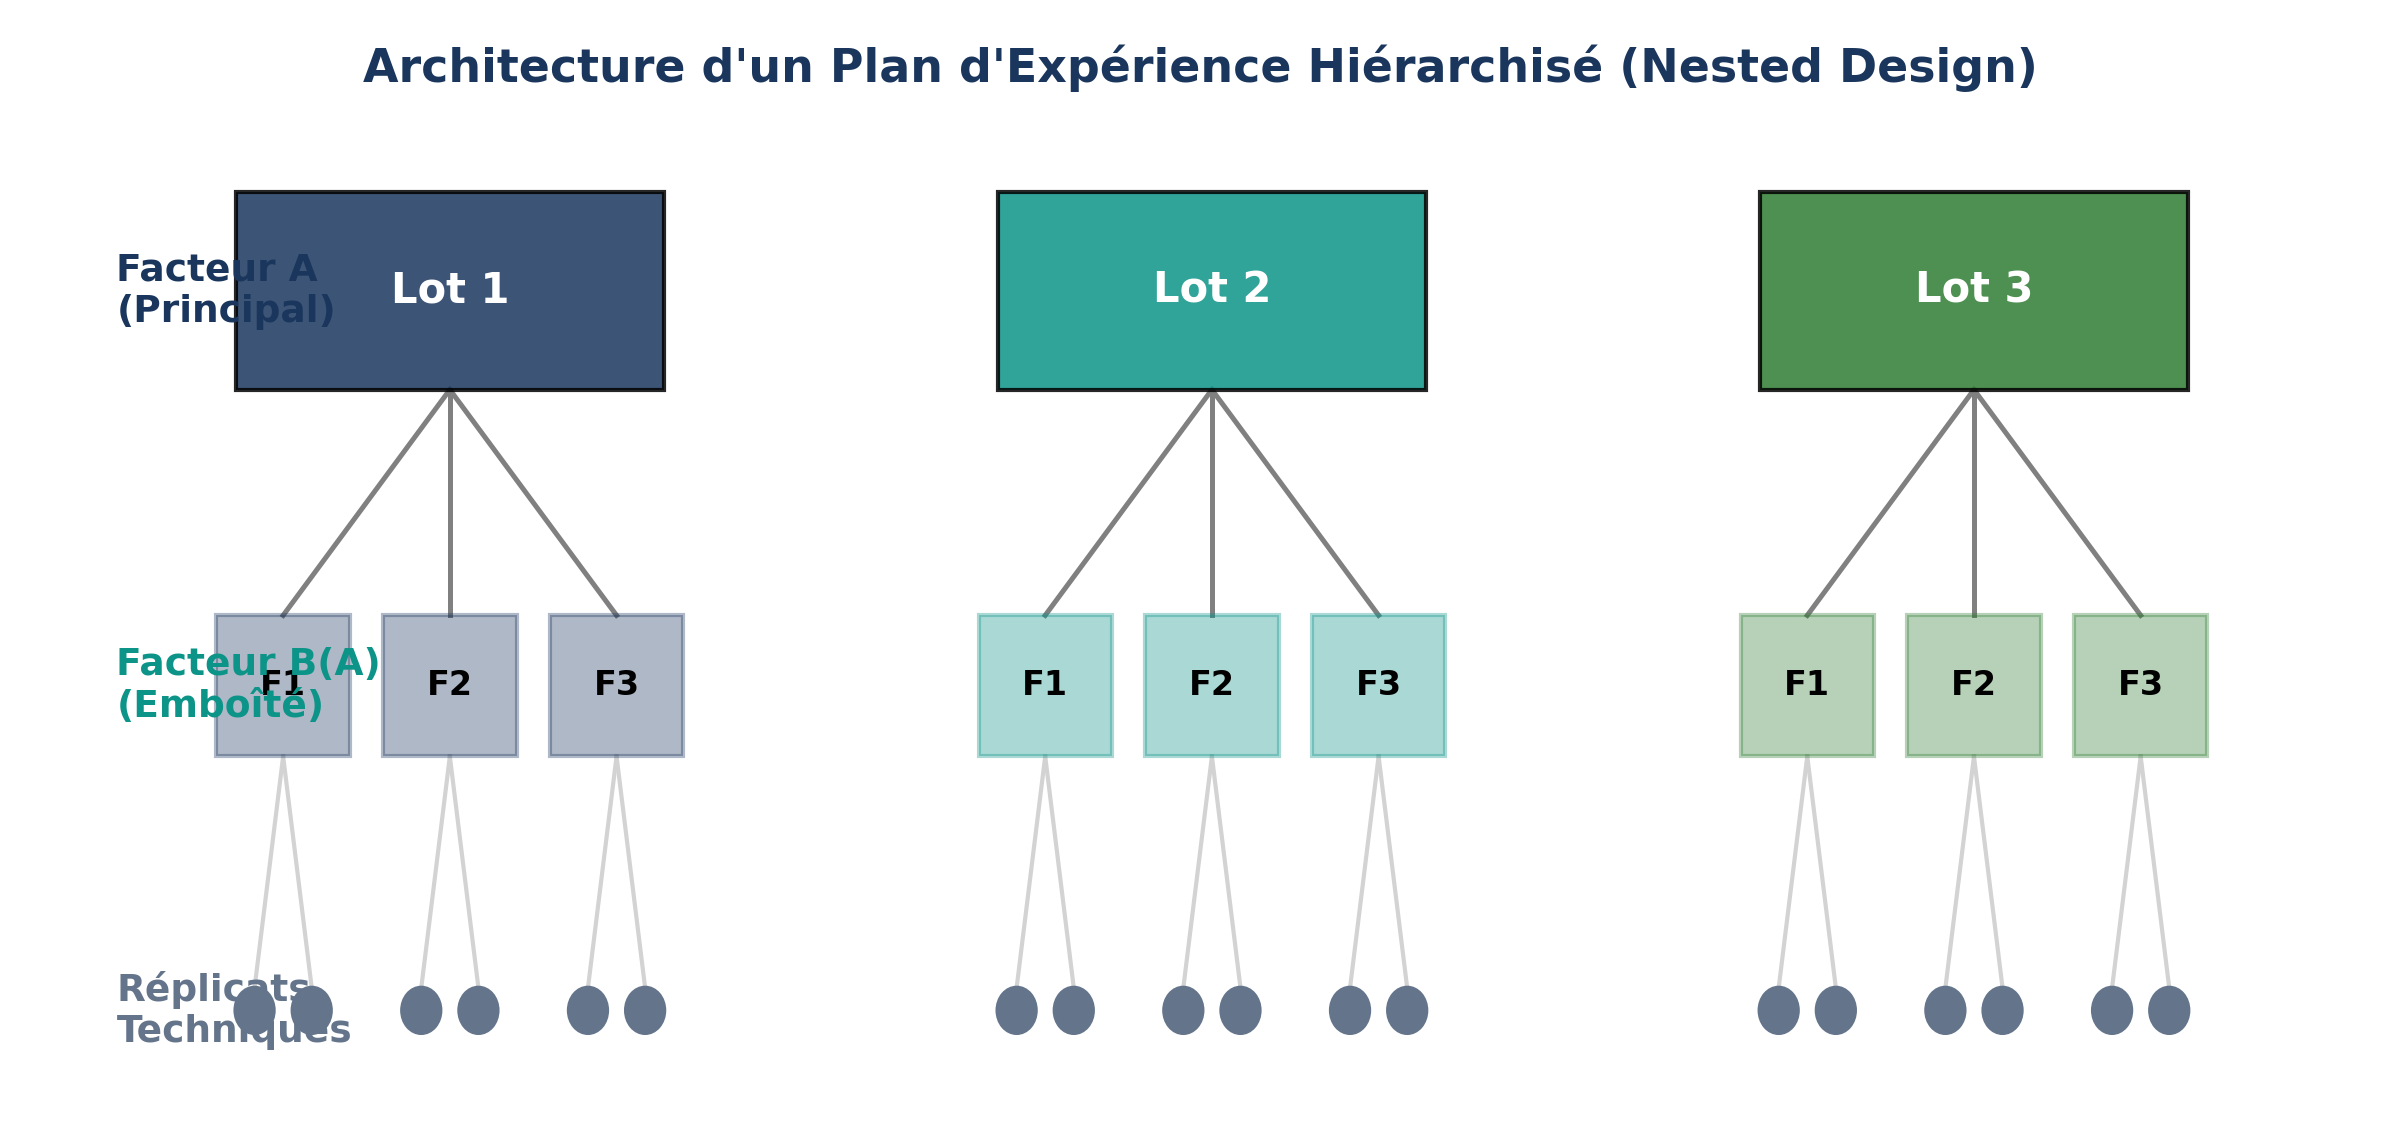
\includegraphics[width=0.88\linewidth]{../figures/fig02_nested_design_tree.png}
  \end{center}
  \vspace{-2mm}
  \begin{takeawaybox}{Structure Hiérarchique à 3 Niveaux}
    Chaque niveau inférieur est contenu dans le niveau supérieur :
    $$\text{Traitement Principal } (A) \longrightarrow \text{Unité Biologique } B(A) \longrightarrow \text{Réplicats Techniques } (k)$$
  \end{takeawaybox}
\end{frame}

% ========================================================
\section{Modélisation \& Choix Crucial du Terme d'Erreur}
% ========================================================

\begin{frame}{Formulation Mathématique du Modèle Hiérarchique}
  \begin{conceptbox}{Équation du Modèle}
    Pour la $k$-ième mesure sur la sous-unité $j$ emboîtée dans le niveau principal $i$ :
    \begin{equation*}
      Y_{ijk} = \mu + \alpha_i + \beta_{j(i)} + \varepsilon_{k(ij)}
    \end{equation*}
  \end{conceptbox}

  \begin{itemize}
    \item $\mu$ : Moyenne générale globale.
    \item $\alpha_i$ : Effet du niveau $i$ du \textbf{Facteur Principal A} ($i = 1, \dots, I$) [généralement à effets fixes].
    \item $\beta_{j(i)}$ : Effet de la sous-unité $j$ \textbf{emboîtée} dans le niveau $i$ ($j = 1, \dots, J$) [généralement à effets aléatoires $\sim \mathcal{N}(0, \sigma_B^2)$].
    \item $\varepsilon_{k(ij)}$ : Erreur technique pure de mesure ($k = 1, \dots, K$) [$\sim \mathcal{N}(0, \sigma^2)$].
  \end{itemize}
\end{frame}

\begin{frame}{La Règle Capitale : Le Bon Dénominateur du Test $F$}
  \begin{table}[h]
    \centering
    \small
    \resizebox{\linewidth}{!}{%
    \begin{tabular}{lcccc}
      \toprule
      \textbf{Source de Variation} & \textbf{$ddl$} & \textbf{Somme des Carrés ($SS$)} & \textbf{Carré Moyen ($MS$)} & \textbf{Statistique $F_{\text{obs}}$} \\
      \midrule
      Facteur Principal A & $I - 1$ & $SS_A$ & $MS_A$ & \cellcolor{BioTeal!25}\textbf{$F_A = \frac{MS_A}{MS_{B(A)}}$} \\
      Facteur Emboîté $B(A)$ & $I(J - 1)$ & $SS_{B(A)}$ & $MS_{B(A)}$ & \cellcolor{BioNavy!10}$F_{B(A)} = \frac{MS_{B(A)}}{MS_{\text{res}}}$ \\
      Erreur Résiduelle Technique & $IJ(K - 1)$ & $SS_{\text{res}}$ & $MS_{\text{res}}$ & --- \\
      \midrule
      \textbf{Total} & $IJK - 1$ & $SS_{\text{Total}}$ & --- & --- \\
      \bottomrule
    \end{tabular}%
    }
  \end{table}

  \begin{takeawaybox}{Pourquoi $F_A = MS_A / MS_{B(A)}$ et NON $MS_A / MS_{\text{res}}$ ?}
    Pour prouver que le Facteur Principal A (ex: Traitement) a un effet réel, sa variabilité $MS_A$ doit dépasser la \textbf{variabilité naturelle entre les individus biologiques} ($MS_{B(A)}$), et non pas seulement la petite erreur de pipetage $MS_{\text{res}}$ ! Diviser par $MS_{\text{res}}$ conduirait à déclarer artificiellement significatif un effet inexistant.
  \end{takeawaybox}
\end{frame}

% ========================================================
\section{Étude de Cas : Bioproduction d'Insuline}
% ========================================================

\begin{frame}{Contrôle Qualité de Pureté d'une Protéine Recombinante}
  \begin{columns}[onlytextwidth, T]
    \begin{column}{0.48\linewidth}
      \begin{biobox}{Procédé Industriel}
        Dans une unité de production biopharmaceutique :
        \begin{itemize}
          \item \textbf{Lots de Fermentation (A) :} 3 bioréacteurs indépendants ($I = 3$).
          \item \textbf{Flacons de Conditionnement (B) :} 3 flacons échantillonnés par lot ($J = 3$).
          \item \textbf{Mesures de Pureté (\%) :} 3 dosages HPLC indépendants par flacon ($K = 3$).
          \item Total : $N = 3 \times 3 \times 3 = 27$ mesures.
        \end{itemize}
      \end{biobox}
    \end{column}
    \begin{column}{0.48\linewidth}
      \begin{conceptbox}{Composantes de la Variance (VCA)}
        Décomposer la variance totale observée :
        \begin{equation*}
          \sigma^2_{\text{totale}} = \sigma^2_{\text{Lot}} + \sigma^2_{\text{Flacon}} + \sigma^2_{\text{HPLC}}
        \end{equation*}
        Permet au directeur qualité d'identifier précisément quel maillon de la chaîne industrielle produit l'hétérogénéité.
      \end{conceptbox}
    \end{column}
  \end{columns}
\end{frame}

\begin{frame}{Résultats de l'ANOVA Hiérarchisée}
  \begin{table}[h]
    \centering
    \small
    \begin{tabular}{lccccc}
      \toprule
      \textbf{Source de Variation} & \textbf{$ddl$} & \textbf{$SS$} & \textbf{$MS$} & \textbf{$F_{\text{obs}}$} & \textbf{$p$-value} \\
      \midrule
      Lots de Production (A) & 2 & 156.24 & 78.12 & \textbf{3.21} & \textbf{0.112} (Non significatif) \\
      Flacons dans Lots $B(A)$ & 6 & 145.80 & 24.30 & \textbf{16.20} & \textbf{$< 0.0001$} (Très significatif) \\
      Erreur Technique HPLC & 18 & 27.00 & 1.50 & --- & --- \\
      \bottomrule
    \end{tabular}
  \end{table}

  \begin{takeawaybox}{Diagnostic \& Décision Industrielle}
    \begin{itemize}
      \item $F_A = \frac{78.12}{24.30} = 3.21$ ($p = 0.112 > 0.05$) : Les 3 grands fermenteurs sont homogènes !
      \item $F_{B(A)} = \frac{24.30}{1.50} = 16.20$ ($p < 0.0001$) : Forte hétérogénéité entre flacons d'un même lot.
      \item $\implies$ \textbf{Conclusion :} La fermentation est maîtrisée. L'anomalie se situe au niveau de la \textbf{ligne de remplissage/bouchage} des flacons. Inutile de reformuler le milieu de culture !
    \end{itemize}
  \end{takeawaybox}
\end{frame}

\begin{frame}[plain]
  \begin{center}
    \vspace{1.8cm}
    {\Huge\color{BioNavy}\textbf{Fin du Chapitre II}}\\[0.8cm]
    {\large Prochaine étape : Corrélation et Régression Linéaire}\\[1.2cm]
    \textbf{Dr. Sarra BENMOUMOU (Ph.D.)}\\
    \small Faculté des Sciences --- Département de Biologie\\
    \textbf{Université M'Hamed Bougara de Boumerdès (UMBB)}
  \end{center}
\end{frame}

\end{document}
